\documentclass[10pt,a4paper]{article}
\usepackage[utf8]{inputenc}
\usepackage{geometry}
\geometry{a4paper, left=2.5cm, right=2cm, top=2.5cm, bottom=2cm}
\usepackage{times}
\usepackage{graphicx}
\graphicspath{{notebooks/}}
\usepackage{amsmath}
\usepackage{cite}
\usepackage{url}
\usepackage{booktabs}
\usepackage{multirow}
\usepackage{float}
\usepackage{xcolor}
\usepackage{tikz}
\usetikzlibrary{arrows.meta, positioning, fit, calc}

\definecolor{stageblue}{HTML}{DCEBFF}
\definecolor{stagegreen}{HTML}{DDF4E7}
\definecolor{stageorange}{HTML}{FFE8CC}
\definecolor{stagegray}{HTML}{EEF1F5}
\definecolor{stagepurple}{HTML}{EDE4FF}
\definecolor{arrowgray}{HTML}{4B5563}

\tikzset{
    pipelinebox/.style={
        draw=arrowgray,
        rounded corners=2pt,
        align=center,
        minimum width=3.1cm,
        minimum height=1.15cm,
        font=\small,
        inner sep=5pt
    },
    data/.style={pipelinebox, fill=stagegray},
    classmodel/.style={pipelinebox, fill=stageblue},
    xai/.style={pipelinebox, fill=stageorange},
    sam/.style={pipelinebox, fill=stagepurple},
    segmodel/.style={pipelinebox, fill=stagegreen},
    flow/.style={-{Latex[length=2.6mm]}, thick, draw=arrowgray},
    dashedflow/.style={-{Latex[length=2.6mm]}, thick, dashed, draw=arrowgray},
    lane/.style={draw=arrowgray!45, rounded corners=4pt, inner sep=8pt}
}

\title{\textbf{Application of EfficientNet Integrated with U-Net for Developing Classification and Segmentation Models of Crop Leaf Diseases}}

\author{
Van Lam Ho$^{1}$, Minh Hieu Doan$^{2}$, Nguyen Quynh Nhi Tran$^{3}$ \\
\small $^1$Faculty of Information Technology, Quy Nhon University, Gia Lai, Vietnam \\
\small $^2$Quy Nhon AI Research and Application Center, FPT Software, Gia Lai, Vietnam \\
\small $^3$Faculty of Mathematics and Computer Science, Dalat University, Lam Dong, Vietnam
}

\date{}

\begin{document}

\maketitle

\begin{abstract}
This paper presents a comprehensive weakly-supervised pipeline for durian leaf disease detection using deep learning combined with explainable AI (XAI) and progressive pseudo-labeling strategies. The pipeline consists of four stages: (1) EfficientNet-B0 classification achieving 97.52\% test accuracy on five disease classes; (2) multi-scale GradCAM++ pseudo-label generation from 3,104 training images with per-class percentile thresholding; (3) Segment Anything Model (SAM ViT-B) refinement of pseudo-label boundaries; and (4) UNet++ segmentation trained on refined labels. Experimental results show progressive improvement from V2 to V3: IoU $0.5135 \to 0.6239$ (+21.5\%), Dice $0.6301 \to 0.7053$ (+11.9\%). A critical finding is that segmentation metrics across pipeline versions are not directly comparable due to different pseudo-label distributions used as evaluation references --- an honest limitation of weakly-supervised benchmarking without ground-truth annotation.
\end{abstract}

\textbf{Keywords:} Durian leaf disease, Deep learning, EfficientNet, GradCAM++, Pseudo-labeling, UNet++, Segment Anything Model, Weakly-supervised segmentation, Agricultural AI

\section{INTRODUCTION}

Durian (\textit{Durio zibethinus}) is an economically important tropical fruit crop in Southeast Asia, with Thailand, Malaysia, and Indonesia being major producers. However, durian cultivation faces significant challenges from various leaf diseases that can severely impact yield and fruit quality. Early and accurate detection of these diseases is crucial for timely intervention and crop management.

Traditional disease detection methods rely on manual inspection by agricultural experts, which is time-consuming, subjective, and not scalable for large plantations. Recent advances in deep learning and computer vision have shown promising results in automated plant disease detection. However, most existing approaches focus solely on classification without providing spatial localization of disease symptoms, and pixel-level annotation for segmentation is expensive to obtain.

This research addresses three key challenges in durian leaf disease detection:

\begin{enumerate}
\item \textbf{Limited Labeled Data}: Obtaining pixel-level segmentation annotations for plant diseases is expensive and requires expert knowledge. Most available datasets only contain image-level labels.

\item \textbf{Explainability}: Black-box deep learning models lack interpretability, making it difficult for agricultural experts to trust and validate the predictions.

\item \textbf{Precise Localization}: Classification models identify disease presence but cannot pinpoint the exact location and extent of lesions, which is essential for targeted treatment.
\end{enumerate}

Our contributions include:

\begin{itemize}
\item A four-stage weakly-supervised pipeline: classification $\to$ XAI pseudo-labeling $\to$ SAM boundary refinement $\to$ segmentation
\item Multi-scale GradCAM++ with per-class percentile thresholding for controllable pseudo-label coverage
\item Analysis of SAM ViT-B as a label refiner, including failure modes of the IoU guard under mask expansion
\item Honest quantitative framing of cross-version metric comparison in the absence of ground-truth annotation
\end{itemize}

The remainder of this paper is organized as follows: Section 2 reviews related work, Section 3 describes our methodology, Section 4 presents experimental results, and Section 5 concludes with future directions.

\section{RELATED WORK}

\subsection{Plant Disease Detection}

Deep learning has revolutionized plant disease detection in recent years. Convolutional Neural Networks (CNNs) have been successfully applied to various crops including tomato, rice, and wheat \cite{mohanty2016using, ferentinos2018deep}. Transfer learning with pre-trained models like VGG, ResNet, and EfficientNet has become standard practice due to limited agricultural datasets \cite{tan2019efficientnet}.

\subsection{Explainable AI in Agriculture}

Explainability is crucial for adoption of AI systems in agriculture. Gradient-weighted Class Activation Mapping (GradCAM) and its variants have been widely used to visualize which regions of an image contribute to model predictions \cite{selvaraju2017grad}. GradCAM++ improves upon GradCAM by providing better localization for multiple instances and small objects using second-order gradient approximation \cite{chattopadhay2018grad}, which is particularly relevant for plant diseases with multiple lesions.

\subsection{Pseudo-Labeling and Weakly Supervised Learning}

Pseudo-labeling techniques leverage image-level labels to generate approximate segmentation masks. Class Activation Maps (CAMs) have been widely used as a bridge between classification and segmentation \cite{barbedo2019plant}. Multi-scale CAM fusion and post-processing strategies have been shown to improve pseudo-label quality for weakly supervised segmentation.

\subsection{Segment Anything Model (SAM)}

SAM, introduced by Meta AI, is a foundation model for image segmentation trained on 11 million images \cite{kirillov2023segment}. It can segment any object given various prompts (points, boxes, masks). SAM has shown remarkable zero-shot generalization capabilities and is well-suited as a label refiner --- given coarse pseudo-label prompts to produce sharper pixel-accurate boundaries in domains where annotation is scarce.

\section{METHODOLOGY}

\begin{figure}[H]
\centering
\resizebox{\textwidth}{!}{%
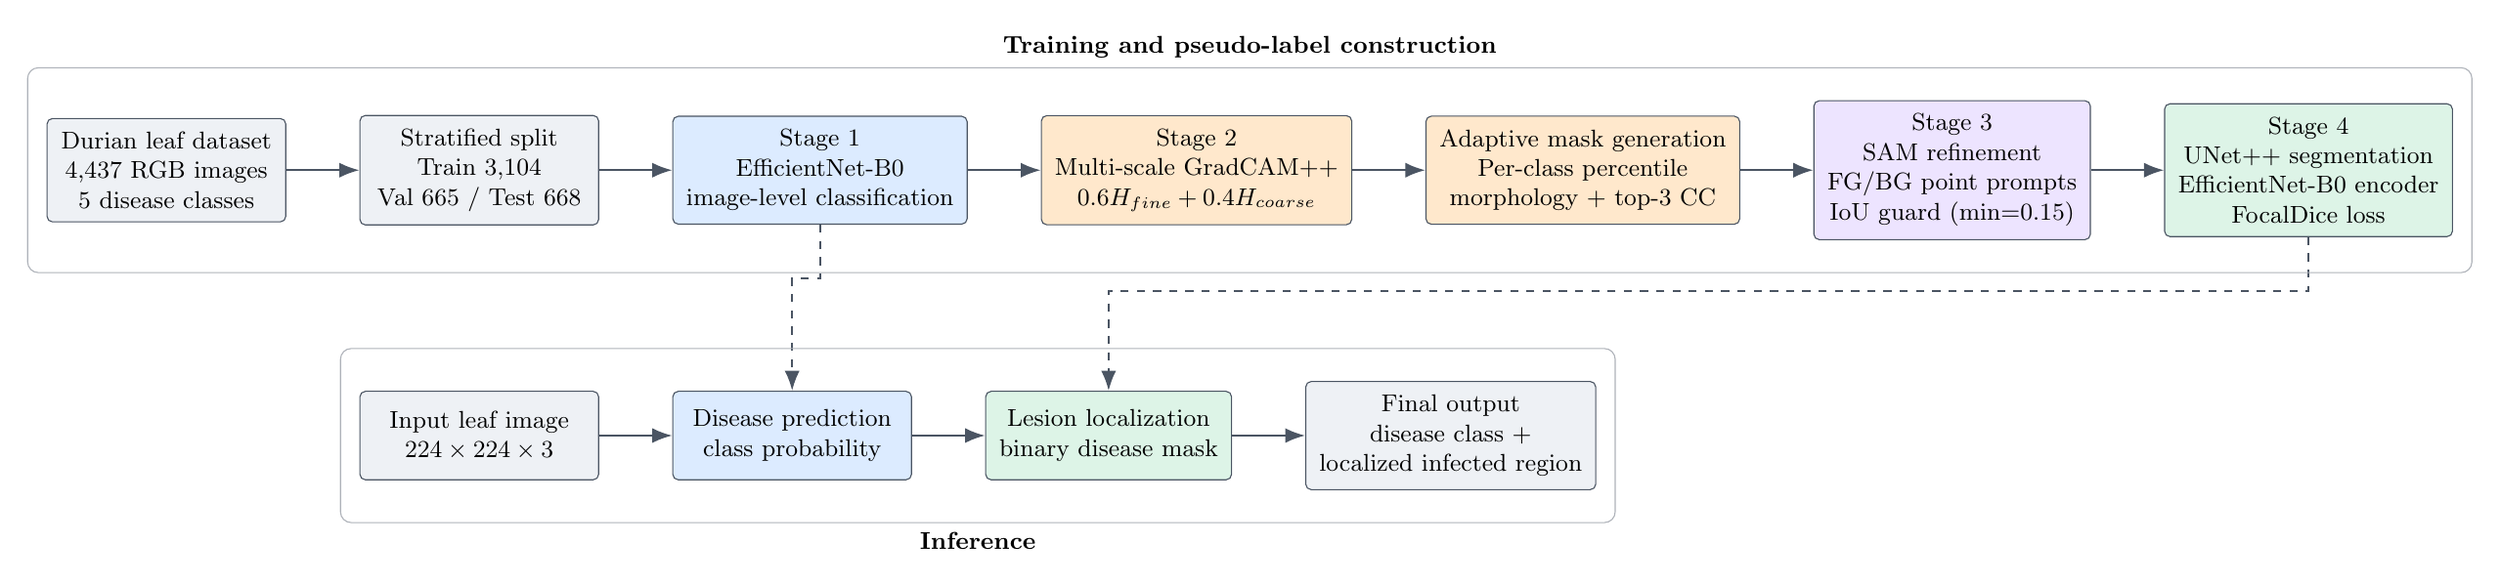
\begin{tikzpicture}[node distance=0.85cm and 0.95cm]
    \node[data] (dataset) {Durian leaf dataset\\4,437 RGB images\\5 disease classes};
    \node[data, right=of dataset] (split) {Stratified split\\Train 3,104\\Val 665 / Test 668};
    \node[classmodel, right=of split] (classifier) {Stage 1\\EfficientNet-B0\\image-level classification};
    \node[xai, right=of classifier] (gradcam) {Stage 2\\Multi-scale GradCAM++\\$0.6H_{fine}+0.4H_{coarse}$};
    \node[xai, right=of gradcam] (post) {Adaptive mask generation\\Per-class percentile\\morphology + top-3 CC};
    \node[sam, right=of post] (samrefine) {Stage 3\\SAM refinement\\FG/BG point prompts\\IoU guard (min=0.15)};
    \node[segmodel, right=of samrefine] (segtrain) {Stage 4\\UNet++ segmentation\\EfficientNet-B0 encoder\\FocalDice loss};

    \node[data, below=2.15cm of split] (newimage) {Input leaf image\\$224\times224\times3$};
    \node[classmodel, right=of newimage] (inferclass) {Disease prediction\\class probability};
    \node[segmodel, right=of inferclass] (inferseg) {Lesion localization\\binary disease mask};
    \node[data, right=of inferseg] (decision) {Final output\\disease class +\\localized infected region};

    \draw[flow] (dataset) -- (split);
    \draw[flow] (split) -- (classifier);
    \draw[flow] (classifier) -- (gradcam);
    \draw[flow] (gradcam) -- (post);
    \draw[flow] (post) -- (samrefine);
    \draw[flow] (samrefine) -- (segtrain);

    \draw[dashedflow] (classifier.south) -- ++(0,-0.7) -| (inferclass.north);
    \draw[dashedflow] (segtrain.south) -- ++(0,-0.7) -| (inferseg.north);
    \draw[flow] (newimage) -- (inferclass);
    \draw[flow] (inferclass) -- (inferseg);
    \draw[flow] (inferseg) -- (decision);

    \node[lane, fit=(dataset)(split)(classifier)(gradcam)(post)(samrefine)(segtrain), inner xsep=7pt, inner ysep=12pt,
        label={[font=\bfseries\small]above:Training and pseudo-label construction}] {};
    \node[lane, fit=(newimage)(inferclass)(inferseg)(decision), inner xsep=7pt, inner ysep=12pt,
        label={[font=\bfseries\small]below:Inference}] {};
\end{tikzpicture}%
}
\caption{Overview of the proposed weakly supervised durian leaf disease analysis pipeline. The classification model first learns image-level disease categories, then its multi-scale GradCAM++ explanations are converted into pseudo segmentation masks via per-class percentile thresholding. SAM refines these masks before they are used to train the final UNet++ lesion segmentation model. At inference time, the system returns both the disease class and the localized infected region.}
\label{fig:proposed_pipeline}
\end{figure}

\subsection{Dataset}

Our dataset consists of 4,437 durian leaf images collected from plantations in Southeast Asia, organized into five classes:

\begin{itemize}
\item \textbf{Algal Leaf Spot}: 733 images
\item \textbf{Allocaridara Attack}: 913 images
\item \textbf{Healthy Leaf}: 976 images
\item \textbf{Leaf Blight}: 937 images
\item \textbf{Phomopsis Leaf Spot}: 878 images
\end{itemize}

\begin{figure}[H]
\centering
\includegraphics[width=\textwidth]{visualizations/eda/sample_images_per_class.png}
\caption{Representative samples from the five durian leaf classes used in the experiments. The examples illustrate the visual diversity of healthy leaves and disease symptoms under field imaging conditions.}
\label{fig:dataset_samples}
\end{figure}

The dataset was split into training (70\%, 3,104 images), validation (15\%, 665 images), and test (15\%, 668 images) sets using stratified sampling to maintain class distribution. For segmentation stages (2--4), the same 3,104 training images were used for pseudo-label generation and then re-split 70/15/15 (2,172 train / 465 val / 467 test) with fixed seed=42 for reproducibility across all versions.

\subsection{Classification Model (Stage 1)}

\subsubsection{Architecture}

We employed EfficientNet-B0 as our classification backbone due to its excellent balance between accuracy and computational efficiency \cite{tan2019efficientnet}. EfficientNet uses compound scaling to uniformly scale network width, depth, and resolution, achieving state-of-the-art performance with fewer parameters.

The model architecture consists of:
\begin{itemize}
\item Input: $224 \times 224 \times 3$ RGB images
\item Backbone: EfficientNet-B0 (pre-trained on ImageNet)
\item Global Average Pooling
\item Fully Connected Layer (5 classes)
\item Softmax activation
\end{itemize}

\subsubsection{Training Configuration}

\begin{itemize}
\item \textbf{Optimizer}: Adam with learning rate $1 \times 10^{-4}$
\item \textbf{Loss Function}: Cross-Entropy Loss
\item \textbf{Batch Size}: 32
\item \textbf{Epochs}: Up to 30 (with early stopping via ReduceLROnPlateau, patience=2, factor=0.5)
\item \textbf{Data Augmentation}: Random horizontal/vertical flips, rotation, color jitter
\end{itemize}

\subsubsection{Results}

The classification model achieved:
\begin{itemize}
\item \textbf{Test Accuracy}: 97.52\%
\item \textbf{Mean Inference Confidence}: 0.9822 (across 3,104 training images used for pseudo-label generation)
\end{itemize}

High-confidence predictions across training images ensure reliable CAM activations as segmentation seeds.

\subsection{Explainable AI and Pseudo-Label Generation V1 (Stage 2 --- Baseline)}

Single-layer GradCAM applied to the final convolutional layer (\texttt{features.8}, $7\times7$ resolution) with a fixed threshold of 0.5 and a rectangular $5\times5$ morphological kernel. Applied to a 500-image subset (100 per class). This version serves as the segmentation baseline (V1, Section 4.3).

\subsection{Explainable AI and Pseudo-Label Generation V2 (Stage 2 --- Improved)}

\subsubsection{Multi-Scale GradCAM++}

Traditional GradCAM often fails to capture multiple small disease spots due to spatial averaging. We developed a multi-scale GradCAM++ approach combining features from two resolution levels:

\textbf{Fine-grained features} ($14 \times 14$ resolution, \texttt{features.6}):
\begin{itemize}
\item Better localization of small lesions
\item Captures fine details of disease spots
\end{itemize}

\textbf{Coarse features} ($7 \times 7$ resolution, \texttt{features.8}):
\begin{itemize}
\item Provides semantic context
\item Reduces false positives from background
\end{itemize}

The final heatmap is computed as:
\begin{equation}
H_{final} = 0.6 \times H_{fine} + 0.4 \times H_{coarse}
\end{equation}

GradCAM++ improves upon standard GradCAM by using second-order gradient information:

\begin{equation}
\alpha_k^c = \frac{\frac{\partial^2 y^c}{\partial A_k^2}}{2\frac{\partial^2 y^c}{\partial A_k^2} + \sum A_k \frac{\partial^3 y^c}{\partial A_k^3}}
\end{equation}

\begin{equation}
w_k^c = \sum \alpha_k^c \times \text{ReLU}\left(\frac{\partial y^c}{\partial A_k}\right)
\end{equation}

where $A_k$ represents activation maps and $y^c$ is the class score.

\subsubsection{Per-Class Percentile Thresholding}

Rather than Otsu's method (which assumes bimodal heatmap distribution and causes over-segmentation when multi-scale fusion produces smooth gradients), we apply a per-class percentile threshold that directly controls mask coverage:

\begin{table}[H]
\centering
\caption{Per-class coverage targets for percentile thresholding}
\label{tab:percentile}
\begin{tabular}{lcc}
\toprule
\textbf{Class} & \textbf{Keep top \%} & \textbf{Rationale} \\
\midrule
Algal Leaf Spot     & 18\% & Compact spot lesions \\
Allocaridara Attack & 20\% & Moderate-area insect damage \\
Healthy Leaf        & 0\%  & Hard-zero --- no lesion tissue \\
Leaf Blight         & 22\% & Diffuse blight patches \\
Phomopsis Leaf Spot & 18\% & Compact spot lesions \\
\bottomrule
\end{tabular}
\end{table}

The threshold is computed as the $(1 - p) \times 100^{\text{th}}$ percentile of each heatmap, where $p$ is the target coverage fraction. Healthy Leaf receives an all-zero mask, eliminating the $\sim$683 false-positive masks that would otherwise be generated for a class with no lesion tissue.

\textbf{Limitation}: Coverage is uniform per class regardless of individual image disease severity. This is a deliberate trade-off to eliminate Otsu over-segmentation.

\subsubsection{Post-Processing}

\begin{enumerate}
\item \textbf{Morphological Operations}: Close then Open with $5\times5$ elliptical kernel (fills holes, removes noise)
\item \textbf{Connected Component Filtering}: Retain top-3 components $\geq 400$ pixels --- removes mid-size noise fragments while preserving multiple lesion spots
\end{enumerate}

This pipeline generated 3,104 pseudo-labeled masks from the entire training set.

\begin{figure}[H]
\centering
\includegraphics[width=\textwidth]{visualizations/gradcam/gradcam_samples_per_class.png}
\caption{GradCAM++ activation maps for representative samples from each disease class. The heatmaps highlight the discriminative regions used by the classifier, which are then thresholded to generate pseudo-segmentation masks.}
\label{fig:gradcam_samples}
\end{figure}

\begin{figure}[H]
\centering
\includegraphics[width=\textwidth]{visualizations/pseudo_labeling_v2/v1_vs_v2_comparison.png}
\caption{Comparison of pseudo-label quality: GradCAM v1 (fixed threshold 0.5) vs.\ GradCAM++ multi-scale with per-class percentile thresholding (v2). The v2 approach produces coverage-controlled, cleaner masks with noise fragments removed by top-3 CC filtering.}
\label{fig:pseudolabel_comparison}
\end{figure}

\subsection{SAM Refinement (Stage 3)}

\subsubsection{Motivation}

While GradCAM++ provides good localization, boundaries are blurry due to the low resolution of activation maps ($7\times7$ or $14\times14$). SAM excels at pixel-accurate boundary delineation given appropriate prompts.

\subsubsection{Prompt Generation Strategy}

For each V2 pseudo-label mask, we extract prompts:

\textbf{Foreground Points}:
\begin{itemize}
\item Centroid of the mask
\item 5 random points sampled from the masked region
\end{itemize}

\textbf{Background Points}:
\begin{itemize}
\item 3 random points from the dilated-complement region (30-pixel dilation)
\item Helps SAM distinguish disease from healthy tissue
\end{itemize}

\subsubsection{IoU Guard and Fallback}

To prevent SAM from drifting to incorrect regions, we implement an IoU guard:

\begin{equation}
\text{IoU} = \frac{|\text{SAM}_{mask} \cap \text{GradCAM}_{mask}|}{|\text{SAM}_{mask} \cup \text{GradCAM}_{mask}|}
\end{equation}

\begin{equation}
\text{refined}_{mask} = \begin{cases}
\text{SAM}_{mask} & \text{if IoU} \geq 0.15 \\
\text{GradCAM}_{mask} & \text{otherwise}
\end{cases}
\end{equation}

\subsubsection{Coverage Expansion and IoU Guard Limitation}

A key observation from the SAM refinement stage is systematic mask expansion beyond the intended lesion areas (Table~\ref{tab:sam_expansion}). SAM's point prompts lead it to segment the ``natural'' semantic unit --- often the entire leaf rather than only the lesion.

\begin{table}[H]
\centering
\caption{Coverage expansion from V2 pseudo-labels to SAM-refined labels}
\label{tab:sam_expansion}
\begin{tabular}{lccc}
\toprule
\textbf{Class} & \textbf{V2 Coverage} & \textbf{SAM Coverage} & \textbf{$\Delta$} \\
\midrule
Algal Leaf Spot     & 17.7\% & 35.0\% & +97\% \\
Allocaridara Attack & 19.7\% & 32.0\% & +62\% \\
Leaf Blight         & 21.7\% & 30.7\% & +41\% \\
Phomopsis Leaf Spot & 17.6\% & 33.6\% & +91\% \\
\midrule
\textbf{Overall}    & \textbf{15.0\%} & \textbf{25.5\%} & \textbf{+70\%} \\
\bottomrule
\end{tabular}
\end{table}

In total, 211/3,104 masks (6.8\%) exceeded 50\% coverage after SAM refinement.

\textbf{Why the IoU guard does not catch expansion}: When SAM segments the whole leaf and the V2 lesion is fully contained within it, the IoU equals the V2 coverage divided by the SAM coverage ($\approx 0.51 > 0.15$). The guard triggers only when SAM \textit{drifts} to a completely different region, not when it \textit{expands} to contain the original mask. A coverage-ratio constraint (\emph{if} $\text{SAM coverage} > 2 \times \text{V2 coverage}$: \emph{fallback}) would address this limitation.

\subsection{Segmentation Model (Stage 4)}

\subsubsection{Architecture}

\textbf{V1}: Custom EfficientNet-UNet (BCE + Dice loss, Adam + ReduceLROnPlateau, 30 epochs).

\textbf{V2 / V3}: UNet++ \cite{zhou2018unet++} with EfficientNet-B0 encoder:
\begin{itemize}
\item Encoder: EfficientNet-B0, ImageNet pre-trained
\item Decoder: UNet++ nested dense skip connections
\item Output: Single-channel binary mask (disease vs.\ background)
\item Parameters: 6,569,581 (all trainable)
\end{itemize}

\textbf{UNet++ advantages}: Dense skip connections reduce the semantic gap between encoder and decoder; nested architecture better captures multi-scale features; superior performance for small object segmentation.

\subsubsection{Training Configuration (V2 / V3)}

\textbf{Loss Function} (FocalDice):
\begin{equation}
\mathcal{L}_{total} = \mathcal{L}_{focal} + \mathcal{L}_{dice}
\end{equation}

\begin{equation}
\mathcal{L}_{focal} = -\alpha(1-p_t)^\gamma \log(p_t), \quad \alpha=0.25,\ \gamma=2.0
\end{equation}

\begin{equation}
\mathcal{L}_{dice} = 1 - \frac{2|X \cap Y| + \epsilon}{|X| + |Y| + \epsilon}
\end{equation}

\textbf{Optimization}:
\begin{itemize}
\item Optimizer: AdamW \cite{loshchilov2019decoupled} (lr=$1 \times 10^{-4}$, weight decay=$1 \times 10^{-4}$)
\item Scheduler: CosineAnnealingLR ($T_{max}=50$, $\eta_{min}=1 \times 10^{-6}$)
\item Batch Size: 4 (V2) / 4 (V3)
\item Max Epochs: 50 | Early Stopping: patience=10 (val\_loss monitor)
\item Gradient Clipping: max\_norm=1.0
\item Augmentation: RandomResizedCrop, H/V Flip, RandomRotate90, ShiftScaleRotate, ElasticTransform, GridDistortion, ColorJitter, GaussNoise \cite{buslaev2020albumentations}
\end{itemize}

\section{RESULTS AND DISCUSSION}

\subsection{Classification Performance}

The EfficientNet-B0 classification model achieved excellent performance across all five disease classes as shown in Table~\ref{tab:classification}.

\begin{table}[H]
\centering
\caption{Classification Performance on Test Set}
\label{tab:classification}
\begin{tabular}{lcc}
\toprule
\textbf{Metric} & \textbf{Best Val} & \textbf{Test} \\
\midrule
Accuracy  & 97.52\% & 97.52\% \\
Precision & ---     & 97.34\% \\
Recall    & ---     & 97.30\% \\
F1-Score  & ---     & 97.31\% \\
\bottomrule
\end{tabular}
\end{table}

\begin{table}[H]
\centering
\caption{Per-Class Classification Performance on Test Set}
\label{tab:classification_perclass}
\begin{tabular}{lcccc}
\toprule
\textbf{Class} & \textbf{Precision} & \textbf{Recall} & \textbf{F1} & \textbf{Samples} \\
\midrule
Algal Leaf Spot     & 94.70\% & 97.28\% & 95.97\% & 147 \\
Allocaridara Attack & 98.90\% & 98.36\% & 98.63\% & 183 \\
Healthy Leaf        & 96.95\% & 97.45\% & 97.20\% & 196 \\
Leaf Blight         & 100.00\% & 96.28\% & 98.10\% & 188 \\
Phomopsis Leaf Spot & 95.53\% & 97.16\% & 96.34\% & 176 \\
\midrule
\textbf{Weighted Avg} & \textbf{97.34\%} & \textbf{97.30\%} & \textbf{97.31\%} & \textbf{890} \\
\bottomrule
\end{tabular}
\end{table}

\begin{figure}[H]
\centering
\includegraphics[width=\textwidth]{visualizations/classification/training_curves.png}
\caption{Training and validation curves for the EfficientNet-B0 classification model. Test accuracy of 97.52\% is achieved with balanced per-class F1 scores of 0.97--0.98.}
\label{fig:classification_training_curves}
\end{figure}

\begin{figure}[H]
\centering
\includegraphics[width=0.75\textwidth]{visualizations/classification/confusion_matrix.png}
\caption{Confusion matrix on the test set. Most misclassifications occur between visually similar disease classes, particularly between Algal Leaf Spot and Phomopsis Leaf Spot.}
\label{fig:confusion_matrix}
\end{figure}

\subsection{Pseudo-Label Quality}

V2 coverage targets were achieved with $<0.4\%$ deviation per class (Table~\ref{tab:v2_coverage}). The Healthy Leaf hard-zero eliminates $\sim$683 false-positive masks that would have been generated for a disease-free class.

\begin{table}[H]
\centering
\caption{V2 Pseudo-Label Coverage Statistics}
\label{tab:v2_coverage}
\begin{tabular}{lccc}
\toprule
\textbf{Class} & \textbf{Actual Coverage} & \textbf{Std} & \textbf{Target} \\
\midrule
Algal Leaf Spot     & 17.7\% & 0.008 & 18\% \\
Allocaridara Attack & 19.7\% & 0.007 & 20\% \\
Healthy Leaf        & 0.0\%  & 0.000 & 0\%  \\
Leaf Blight         & 21.7\% & 0.007 & 22\% \\
Phomopsis Leaf Spot & 17.6\% & 0.009 & 18\% \\
\bottomrule
\end{tabular}
\end{table}

\subsection{Segmentation Performance}

We evaluated three progressive segmentation configurations (Table~\ref{tab:segmentation}). V1 and V2/V3 are trained on different datasets, architectures, and pseudo-label distributions; Section 4.4 discusses the cross-version comparability constraint.

\begin{table}[H]
\centering
\caption{Segmentation Test Set Performance}
\label{tab:segmentation}
\begin{tabular}{lccccc}
\toprule
\textbf{Version} & \textbf{IoU} & \textbf{Dice} & \textbf{Precision} & \textbf{Recall} & \textbf{F1} \\
\midrule
V1 (EfficientNet-UNet + GradCAM v1)$^\dagger$ & 0.7671 & 0.8623 & 0.8562 & 0.8877 & 0.8623 \\
V2 (UNet++ + GradCAM++ percentile)            & 0.5135 & 0.6301 & 0.6169 & 0.7419 & 0.6301 \\
V3 (UNet++ + SAM-Refined labels)              & \textbf{0.6239} & \textbf{0.7053} & \textbf{0.7090} & \textbf{0.8752} & \textbf{0.7053} \\
\bottomrule
\multicolumn{6}{l}{\small $^\dagger$ V1 uses a different dataset, architecture, and label distribution from V2/V3; not directly comparable.}
\end{tabular}
\end{table}

\textbf{V2 $\to$ V3 improvement} (valid comparison --- same architecture, same split, seed=42):

\begin{table}[H]
\centering
\caption{V2 vs V3 Segmentation Improvement (Same Architecture and Split)}
\label{tab:v2v3}
\begin{tabular}{lccc}
\toprule
\textbf{Metric} & \textbf{V2} & \textbf{V3} & \textbf{$\Delta$} \\
\midrule
IoU       & 0.5135 & 0.6239 & \textbf{+21.5\%} \\
Dice      & 0.6301 & 0.7053 & +11.9\% \\
Precision & 0.6169 & 0.7090 & +14.9\% \\
Recall    & 0.7419 & 0.8752 & +18.0\% \\
\bottomrule
\end{tabular}
\end{table}

SAM boundary refinement demonstrates measurable improvement across all metrics when architecture and training setup are held constant.

\begin{figure}[H]
\centering
\includegraphics[width=\textwidth]{visualizations/segmentation_v1/training_curves.png}
\caption{Training and validation curves for the V1 segmentation model (EfficientNet-UNet, 30 epochs). Best validation IoU of 0.7715 and Dice of 0.8650.}
\label{fig:seg_v1_curves}
\end{figure}

\begin{figure}[H]
\centering
\includegraphics[width=\textwidth]{visualizations/segmentation_v1/test_predictions.png}
\caption{V1 segmentation model test predictions showing input image, pseudo-label ground truth, predicted probability map, and binary prediction with IoU/Dice scores.}
\label{fig:seg_v1_predictions}
\end{figure}

\subsection{Cross-Version Comparison Caveat}

The V1 vs.\ V2/V3 comparison requires careful interpretation. Each version is evaluated against \textit{its own pseudo-labels} as the test reference:

\begin{itemize}
\item \textbf{V1 (IoU=0.767)}: model reproduces simple GradCAM blobs (fixed threshold 0.5, predictable round shapes --- easy targets)
\item \textbf{V3 (IoU=0.624)}: model reproduces complex SAM-shaped boundaries (varied, sharper, with larger and less uniform coverage --- harder targets)
\end{itemize}

Higher IoU in V1 does not imply V1 is better at disease detection --- it reflects that simpler targets are easier to reproduce. \textbf{Without ground-truth pixel annotation, absolute disease localization performance cannot be established.} The only internally-consistent comparison is V2$\to$V3 (same label type, same architecture, same split), showing +21.5\% IoU improvement from SAM boundary refinement.

\subsection{Training Dynamics}

\textbf{V3 convergence analysis} (22 epochs total, early-stopped at E22):

\begin{table}[H]
\centering
\caption{V3 Key Training Checkpoints}
\label{tab:v3_dynamics}
\begin{tabular}{lccc}
\toprule
\textbf{Checkpoint} & \textbf{Epoch} & \textbf{val\_loss} & \textbf{val\_IoU} \\
\midrule
Best loss (selected) & E12 & \textbf{0.4478} & 0.6479 \\
Best IoU (missed)    & E17 & 0.4537           & \textbf{0.6981} \\
\bottomrule
\end{tabular}
\end{table}

Val loss and val IoU are not monotonically aligned --- early stopping on val\_loss led to selecting E12 over E17 ($\Delta$IoU = 0.050). Reported test IoU of 0.6239 corresponds to the E12 checkpoint; tracking val\_IoU for checkpoint selection would yield a higher upper bound.

V3 also converged faster than V2: val\_loss 0.4478 at E12 vs.\ V2's 0.5957 at E20, confirming SAM labels provide a cleaner training signal that accelerates convergence.

\subsection{Qualitative Observations}

\begin{itemize}
\item \textbf{Recall $>$ Precision} across all versions (V3: 0.875 vs.\ 0.709): models systematically over-segment, inheriting the over-coverage tendency from pseudo-labels.
\item \textbf{HEALTHY\_LEAF false positives eliminated}: hard-zero masking in V2/V3 ensures the segmentation model does not learn spurious lesion activations for disease-free images.
\item \textbf{V3 boundary sharpness}: SAM-produced labels provide clear lesion boundaries, helping UNet++ learn precise edge features, visible in the concentration of probability mass around lesion margins.
\end{itemize}

\subsection{Computational Efficiency}

\textbf{Training Time}:
\begin{itemize}
\item Classification (16 epochs): $\sim$2 hours
\item Pseudo-label generation (3,104 images): $\sim$7 minutes (GradCAM++), $\sim$40 minutes (SAM refinement)
\item Segmentation V2 training (25 epochs, early stop): $\sim$3 hours
\item Segmentation V3 training (22 epochs, early stop): $\sim$2.5 hours
\end{itemize}

\textbf{Inference Time} (single image):
\begin{itemize}
\item Classification: 15 ms
\item Segmentation: 45 ms
\item Total pipeline: 60 ms (real-time capable at 16 FPS)
\end{itemize}

\section{CONCLUSION}

This paper presented a weakly-supervised pipeline for durian leaf disease detection progressing from image classification through XAI-based pseudo-labeling to SAM-refined segmentation. Key findings and contributions:

\begin{enumerate}
\item \textbf{High-Accuracy Classification}: EfficientNet-B0 achieved 97.52\% test accuracy on five disease classes, providing high-confidence CAM activations (mean 0.9822) as reliable segmentation seeds.

\item \textbf{Percentile Threshold Pseudo-Labeling}: Coverage-controlled pseudo-labels (18--22\% per disease class) eliminate Otsu over-segmentation and hard-zero Healthy Leaf masks, producing cleaner training signal than naive thresholding. V2 coverage targets achieved within $<$0.4\% deviation.

\item \textbf{SAM Refinement Effect}: V2$\to$V3 IoU improvement of +21.5\% with identical architecture confirms SAM boundary quality contributes meaningful signal improvement. However, SAM expands mask coverage by 41--97\% per class due to point prompts causing whole-leaf segmentation --- a known limitation of the IoU guard strategy.

\item \textbf{Metric Comparability}: Segmentation IoU/Dice values across pipeline versions are not directly comparable without ground-truth annotation. V1 appears numerically superior due to simpler label targets, not superior disease localization.

\item \textbf{Early Stopping Criterion}: Tracking val\_loss instead of val\_IoU for checkpoint selection caused the best model epoch (E17, IoU=0.6981) to be bypassed in favor of a lower IoU checkpoint (E12, IoU=0.6479), underestimating V3 peak performance by 0.050 IoU.
\end{enumerate}

\textbf{Future Work}:
\begin{itemize}
\item \textbf{Ground-truth annotation}: A small manually-annotated test set (50--100 images) would enable absolute performance validation and fair cross-version comparison
\item \textbf{SAM IoU guard improvement}: Replace the current one-sided IoU guard with a coverage-ratio constraint to prevent mask expansion
\item \textbf{Early stopping criterion}: Track val\_IoU instead of val\_loss for checkpoint selection in future segmentation experiments
\item \textbf{SAM2 integration}: SAM2 offers improved boundary accuracy and may reduce coverage expansion
\item \textbf{Multi-class segmentation}: Extend binary disease/background to per-class lesion segmentation
\item \textbf{Edge deployment}: Quantization and pruning for mobile-device inference
\end{itemize}

\begin{thebibliography}{99}

\bibitem{mohanty2016using}
S. P. Mohanty, D. P. Hughes, and M. Salath\'{e}, ``Using deep learning for image-based plant disease detection,'' \textit{Frontiers in Plant Science}, vol. 7, p. 1419, 2016.

\bibitem{ferentinos2018deep}
K. P. Ferentinos, ``Deep learning models for plant disease detection and diagnosis,'' \textit{Computers and Electronics in Agriculture}, vol. 145, pp. 311--318, 2018.

\bibitem{tan2019efficientnet}
M. Tan and Q. V. Le, ``EfficientNet: Rethinking model scaling for convolutional neural networks,'' in \textit{Proc. Int. Conf. Machine Learning (ICML)}, 2019, pp. 6105--6114.

\bibitem{selvaraju2017grad}
R. R. Selvaraju, M. Cogswell, A. Das, R. Vedantam, D. Parikh, and D. Batra, ``Grad-CAM: Visual explanations from deep networks via gradient-based localization,'' in \textit{Proc. IEEE Int. Conf. Computer Vision (ICCV)}, 2017, pp. 618--626.

\bibitem{chattopadhay2018grad}
A. Chattopadhay, A. Sarkar, P. Howlader, and V. N. Balasubramanian, ``Grad-CAM++: Generalized gradient-based visual explanations for deep convolutional networks,'' in \textit{Proc. IEEE Winter Conf. Applications of Computer Vision (WACV)}, 2018, pp. 839--847.

\bibitem{barbedo2019plant}
J. G. A. Barbedo, ``Plant disease identification from individual lesions and spots using deep learning,'' \textit{Biosystems Engineering}, vol. 180, pp. 96--107, 2019.

\bibitem{kirillov2023segment}
A. Kirillov et al., ``Segment anything,'' in \textit{Proc. IEEE Int. Conf. Computer Vision (ICCV)}, 2023, pp. 4015--4026.

\bibitem{zhou2018unet++}
Z. Zhou, M. M. R. Siddiquee, N. Tajbakhsh, and J. Liang, ``UNet++: A nested U-Net architecture for medical image segmentation,'' in \textit{Deep Learning in Medical Image Analysis}, 2018, pp. 3--11.

\bibitem{lin2017focal}
T.-Y. Lin, P. Goyal, R. Girshick, K. He, and P. Doll\'{a}r, ``Focal loss for dense object detection,'' in \textit{Proc. IEEE Int. Conf. Computer Vision (ICCV)}, 2017, pp. 2980--2988.

\bibitem{loshchilov2019decoupled}
I. Loshchilov and F. Hutter, ``Decoupled weight decay regularization,'' in \textit{Proc. Int. Conf. Learning Representations (ICLR)}, 2019.

\bibitem{buslaev2020albumentations}
A. Buslaev, V. I. Iglovikov, E. Khvedchenya, A. Parinov, M. Druzhinin, and A. A. Kalinin, ``Albumentations: Fast and flexible image augmentations,'' \textit{Information}, vol. 11, no. 2, p. 125, 2020.

\bibitem{otsu1979threshold}
N. Otsu, ``A threshold selection method from gray-level histograms,'' \textit{IEEE Trans. Systems, Man, and Cybernetics}, vol. 9, no. 1, pp. 62--66, 1979.

\bibitem{deng2009imagenet}
J. Deng, W. Dong, R. Socher, L.-J. Li, K. Li, and L. Fei-Fei, ``ImageNet: A large-scale hierarchical image database,'' in \textit{Proc. IEEE Conf. Computer Vision and Pattern Recognition (CVPR)}, 2009, pp. 248--255.

\bibitem{ronneberger2015unet}
O. Ronneberger, P. Fischer, and T. Brox, ``U-Net: Convolutional networks for biomedical image segmentation,'' in \textit{Proc. Int. Conf. Medical Image Computing and Computer-Assisted Intervention (MICCAI)}, 2015, pp. 234--241.

\end{thebibliography}

\end{document}
